\begin{figure*}[!hbt]
  \centering
  \subfigure[Runtime on consecutive batch updates of size $10^{-5}|E_T|$]{
    \label{fig:temporal-sx-mathoverflow--runtime5}
    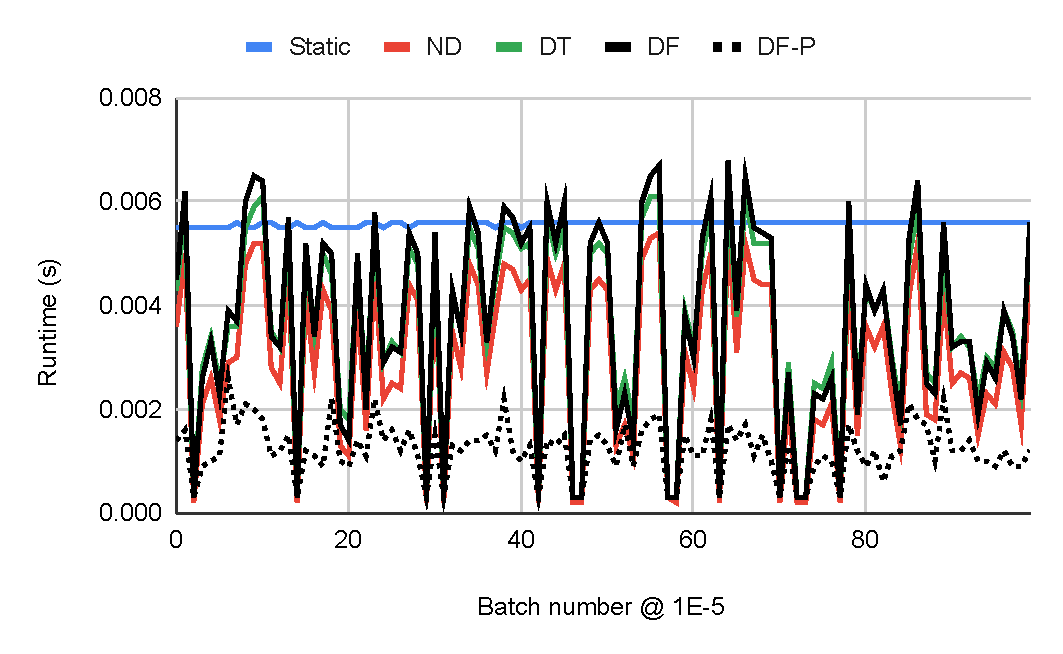
\includegraphics[width=0.48\linewidth]{out/temporal-sx-mathoverflow-runtime5.pdf}
  }
  \subfigure[Error in ranks obtained on consecutive batch updates of size $10^{-5}|E_T|$]{
    \label{fig:temporal-sx-mathoverflow--error5}
    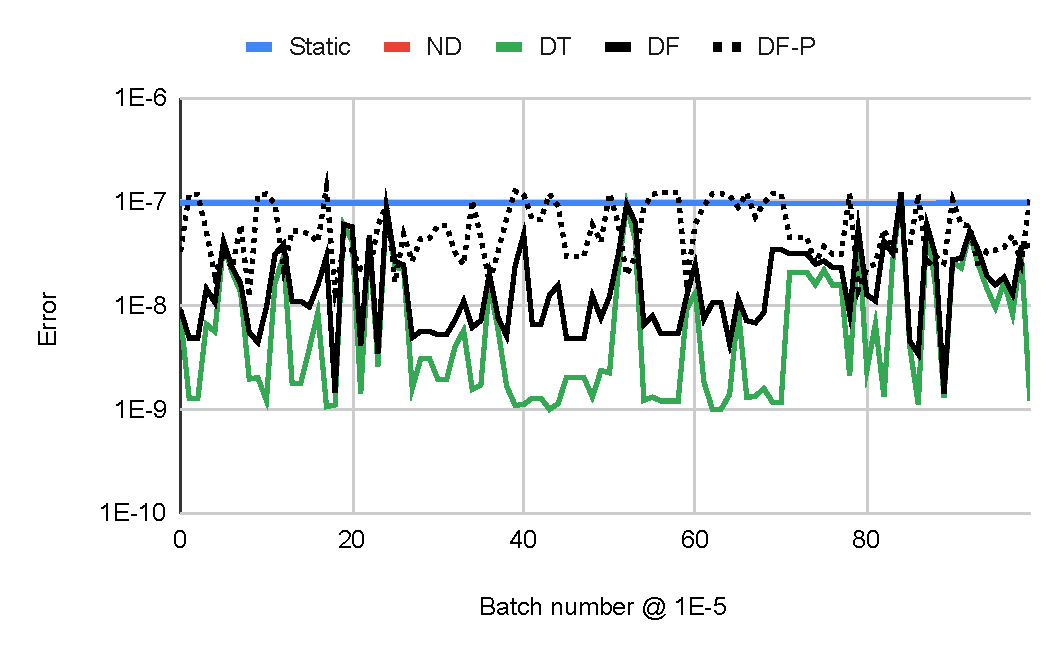
\includegraphics[width=0.48\linewidth]{out/temporal-sx-mathoverflow-error5.pdf}
  } \\[2ex]
  \subfigure[Runtime on consecutive batch updates of size $10^{-4}|E_T|$]{
    \label{fig:temporal-sx-mathoverflow--runtime4}
    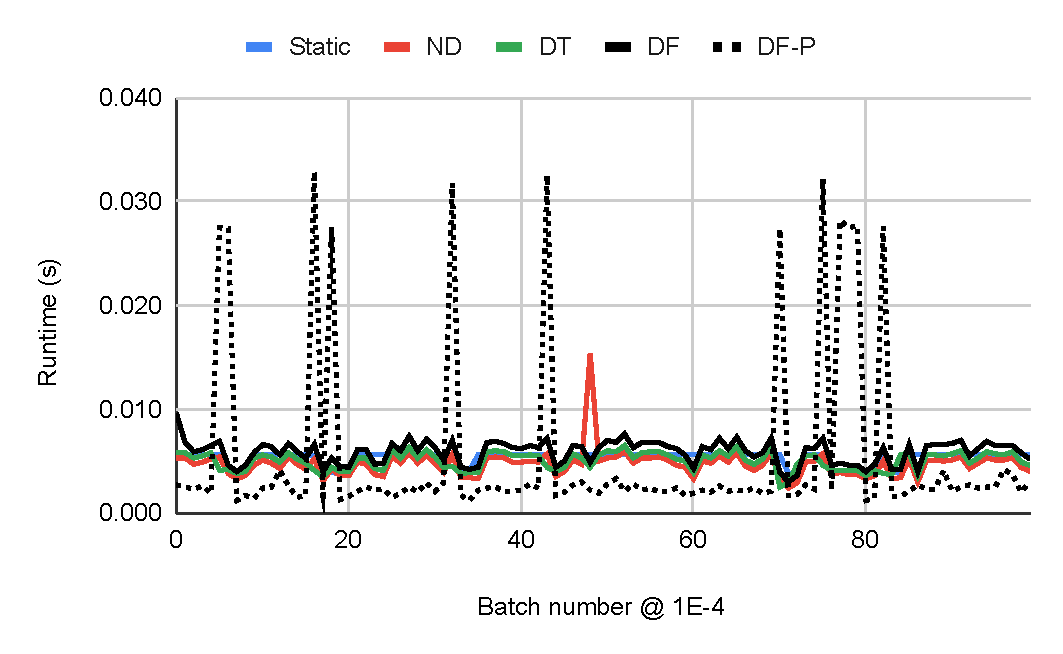
\includegraphics[width=0.48\linewidth]{out/temporal-sx-mathoverflow-runtime4.pdf}
  }
  \subfigure[Error in ranks obtained on consecutive batch updates of size $10^{-4}|E_T|$]{
    \label{fig:temporal-sx-mathoverflow--error4}
    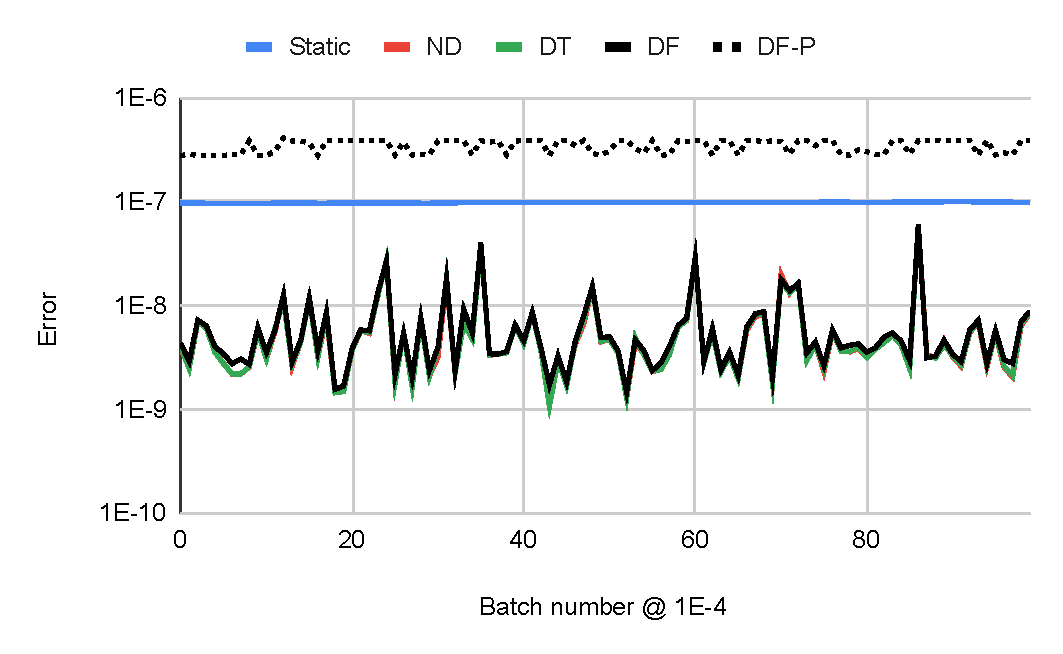
\includegraphics[width=0.48\linewidth]{out/temporal-sx-mathoverflow-error4.pdf}
  } \\[2ex]
  \subfigure[Runtime on consecutive batch updates of size $10^{-3}|E_T|$]{
    \label{fig:temporal-sx-mathoverflow--runtime3}
    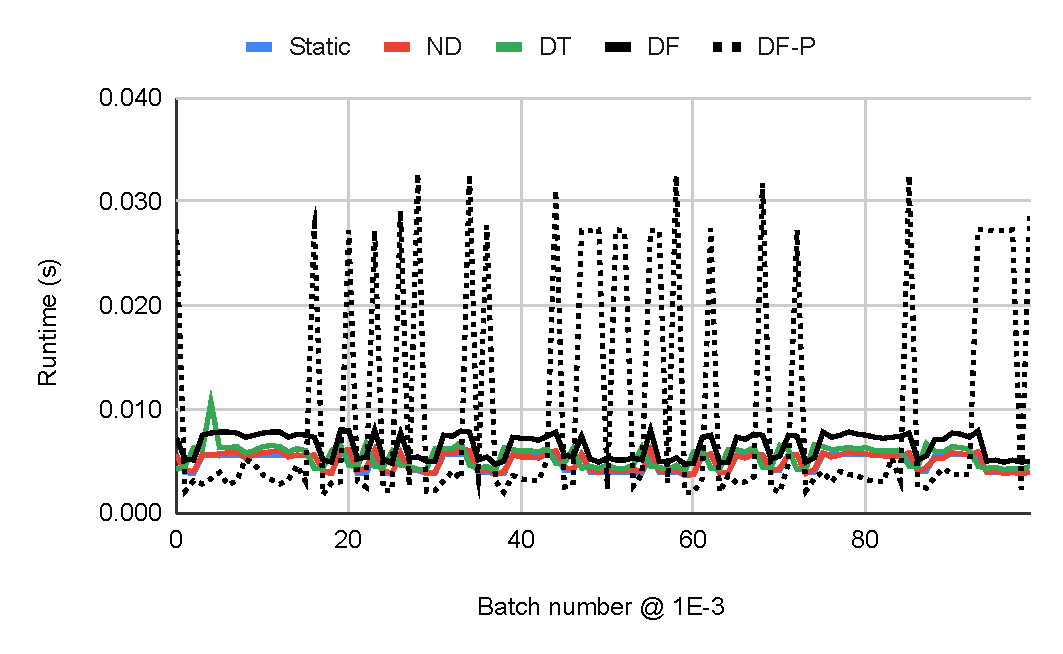
\includegraphics[width=0.48\linewidth]{out/temporal-sx-mathoverflow-runtime3.pdf}
  }
  \subfigure[Error in ranks obtained on consecutive batch updates of size $10^{-3}|E_T|$]{
    \label{fig:temporal-sx-mathoverflow--error3}
    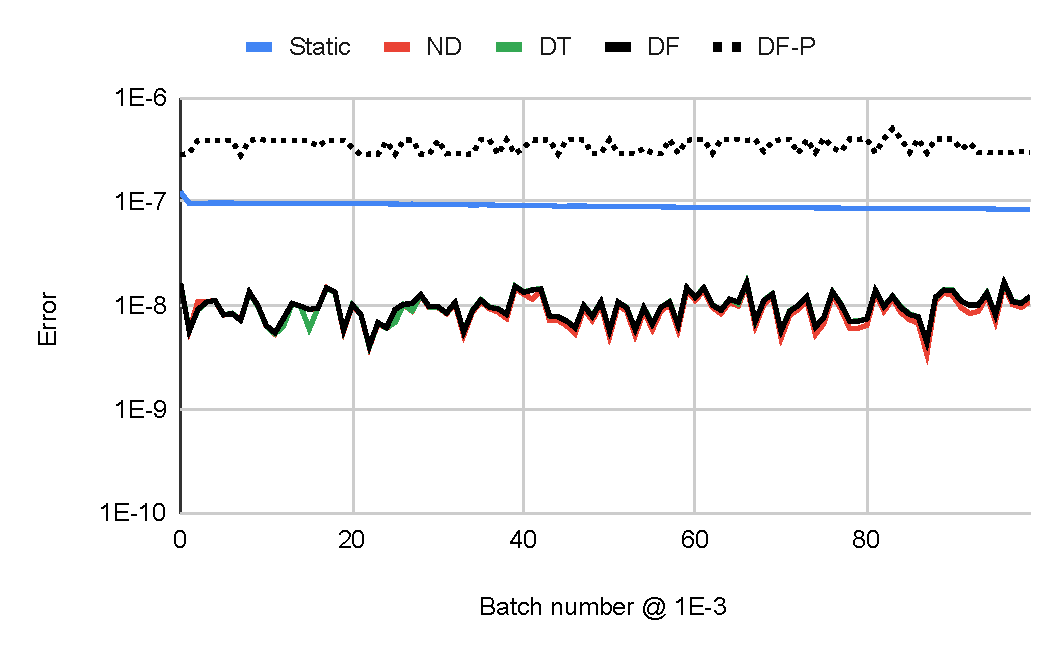
\includegraphics[width=0.48\linewidth]{out/temporal-sx-mathoverflow-error3.pdf}
  } \\[-2ex]
  \caption{Runtime and Error in ranks obtained with \textit{Static}, \textit{Naive-dynamic (ND)}, \textit{Dynamic Traversal (DT)}, our improved \textit{Dynamic Frontier (DF)}, and our improved \textit{Dynamic Frontier with Pruning (DF-P)} PageRank on the \textit{sx-mathoverflow} dynamic graph. The size of batch updates range from $10^{-5}|E_T|$ to $10^{-3}|E_T|$. The rank error with each approach is measured relative to ranks obtained with a reference Static PageRank run, as detailed in Section \ref{sec:measurement}. \su{TOWR}}
  \label{fig:temporal-sx-mathoverflow}
\end{figure*}

\begin{figure*}[!hbt]
  \centering
  \subfigure[Runtime on consecutive batch updates of size $10^{-5}|E_T|$]{
    \label{fig:temporal-sx-askubuntu--runtime5}
    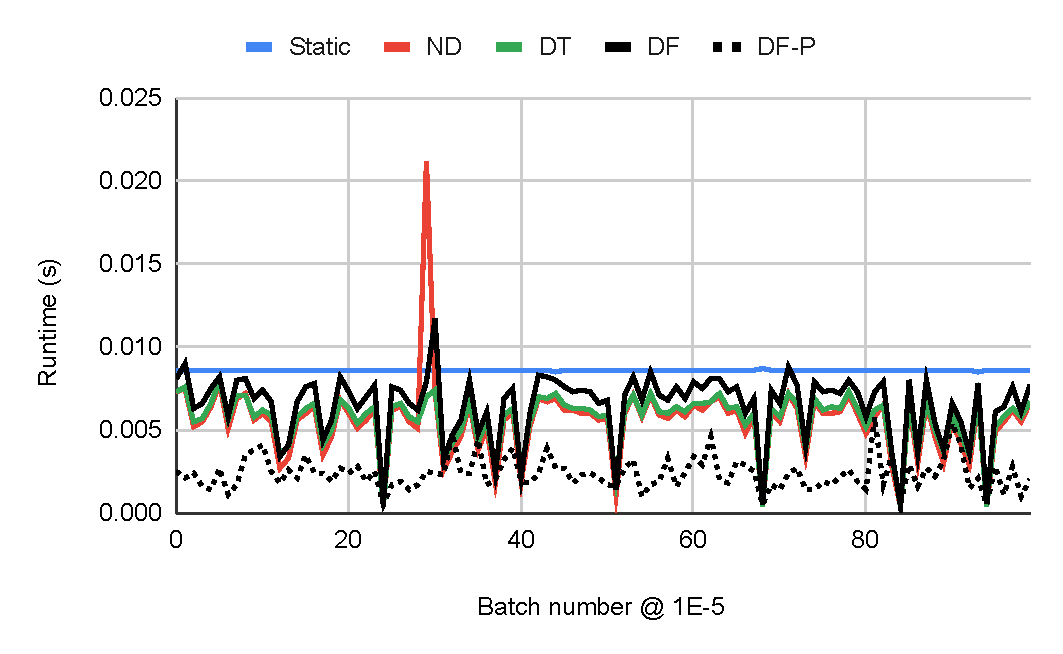
\includegraphics[width=0.48\linewidth]{out/temporal-sx-askubuntu-runtime5.pdf}
  }
  \subfigure[Error in ranks obtained on consecutive batch updates of size $10^{-5}|E_T|$]{
    \label{fig:temporal-sx-askubuntu--error5}
    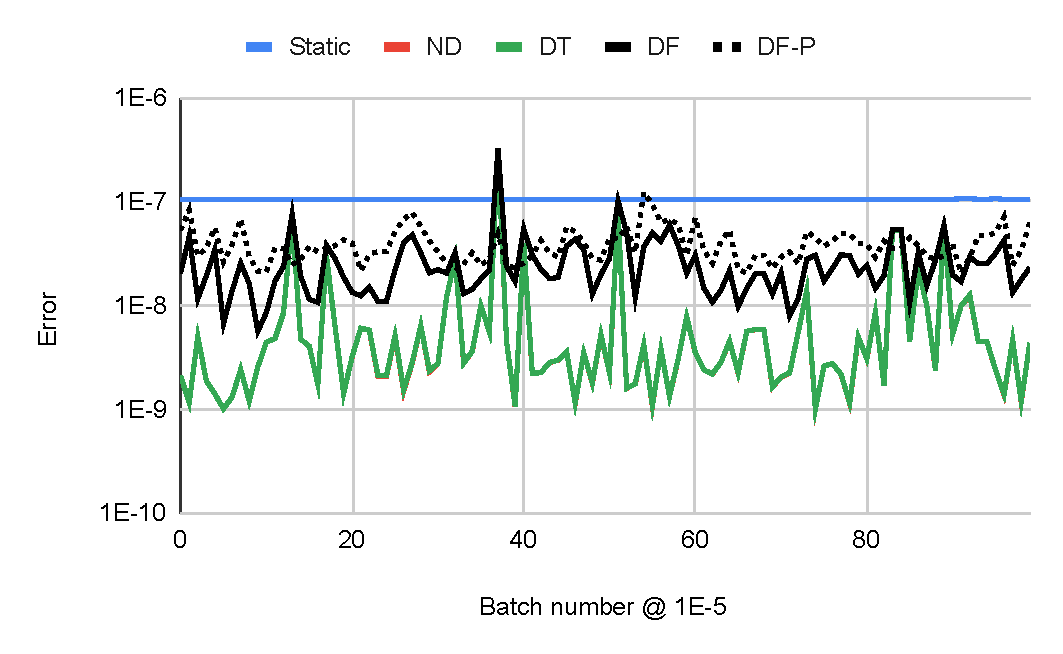
\includegraphics[width=0.48\linewidth]{out/temporal-sx-askubuntu-error5.pdf}
  } \\[2ex]
  \subfigure[Runtime on consecutive batch updates of size $10^{-4}|E_T|$]{
    \label{fig:temporal-sx-askubuntu--runtime4}
    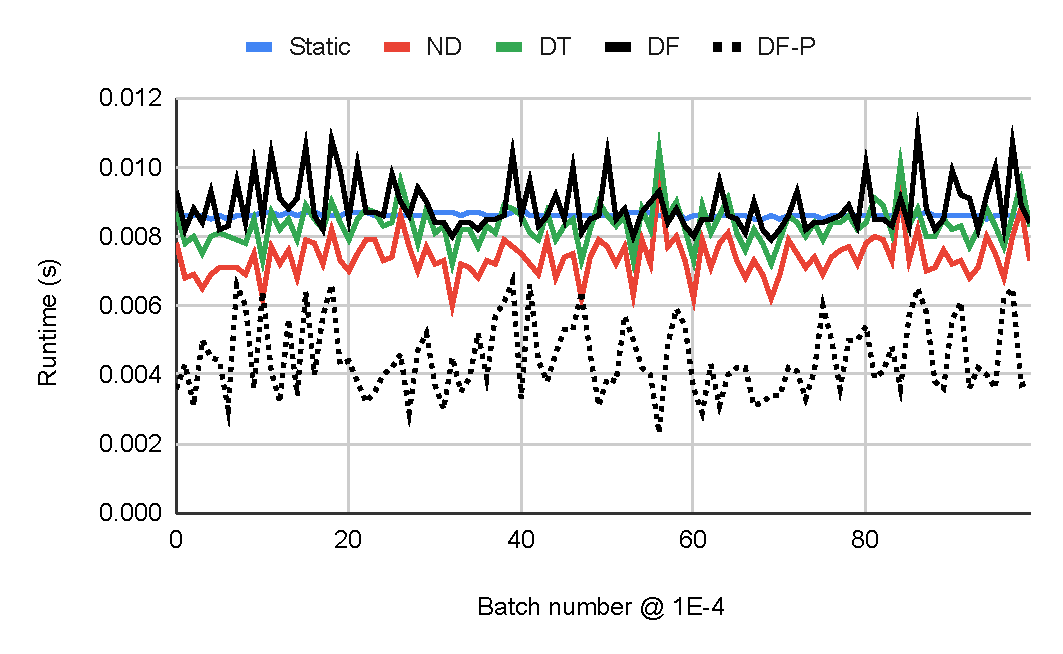
\includegraphics[width=0.48\linewidth]{out/temporal-sx-askubuntu-runtime4.pdf}
  }
  \subfigure[Error in ranks obtained on consecutive batch updates of size $10^{-4}|E_T|$]{
    \label{fig:temporal-sx-askubuntu--error4}
    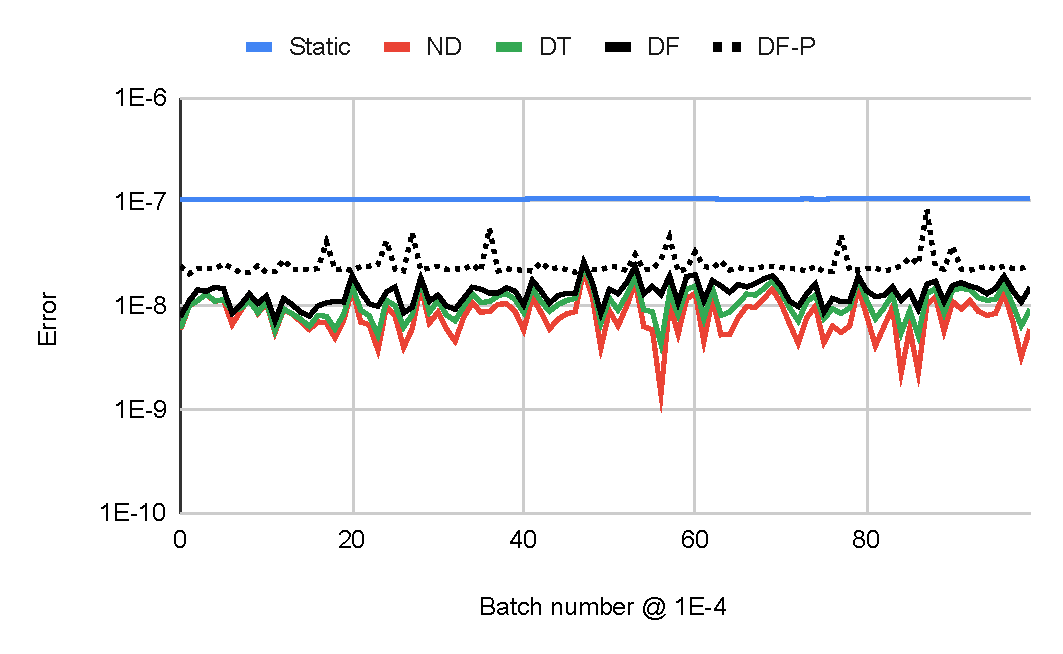
\includegraphics[width=0.48\linewidth]{out/temporal-sx-askubuntu-error4.pdf}
  } \\[2ex]
  \subfigure[Runtime on consecutive batch updates of size $10^{-3}|E_T|$]{
    \label{fig:temporal-sx-askubuntu--runtime3}
    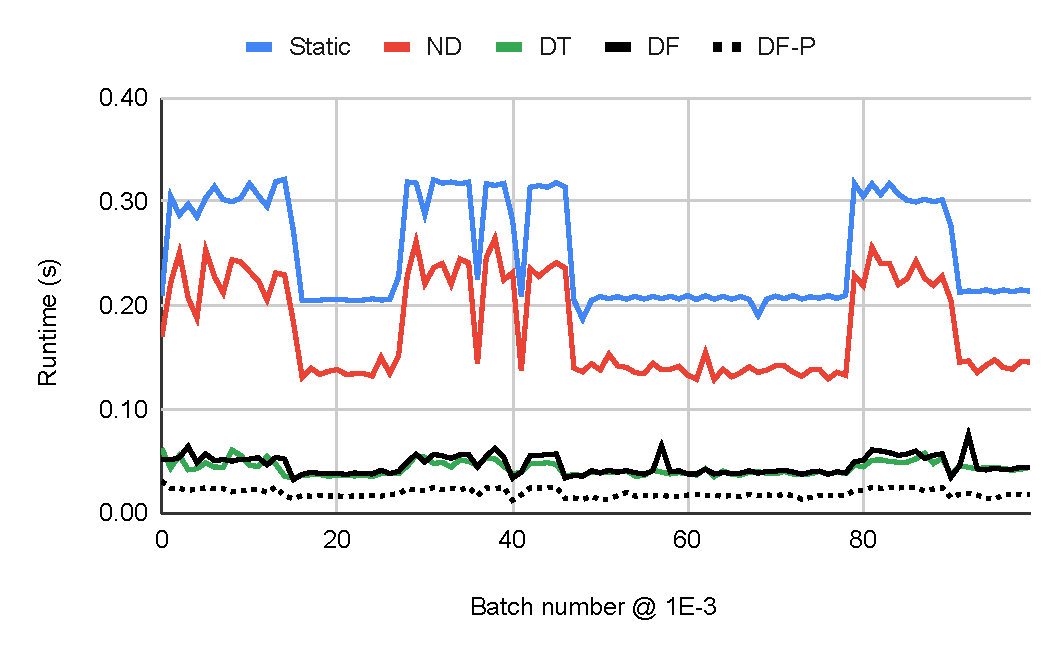
\includegraphics[width=0.48\linewidth]{out/temporal-sx-askubuntu-runtime3.pdf}
  }
  \subfigure[Error in ranks obtained on consecutive batch updates of size $10^{-3}|E_T|$]{
    \label{fig:temporal-sx-askubuntu--error3}
    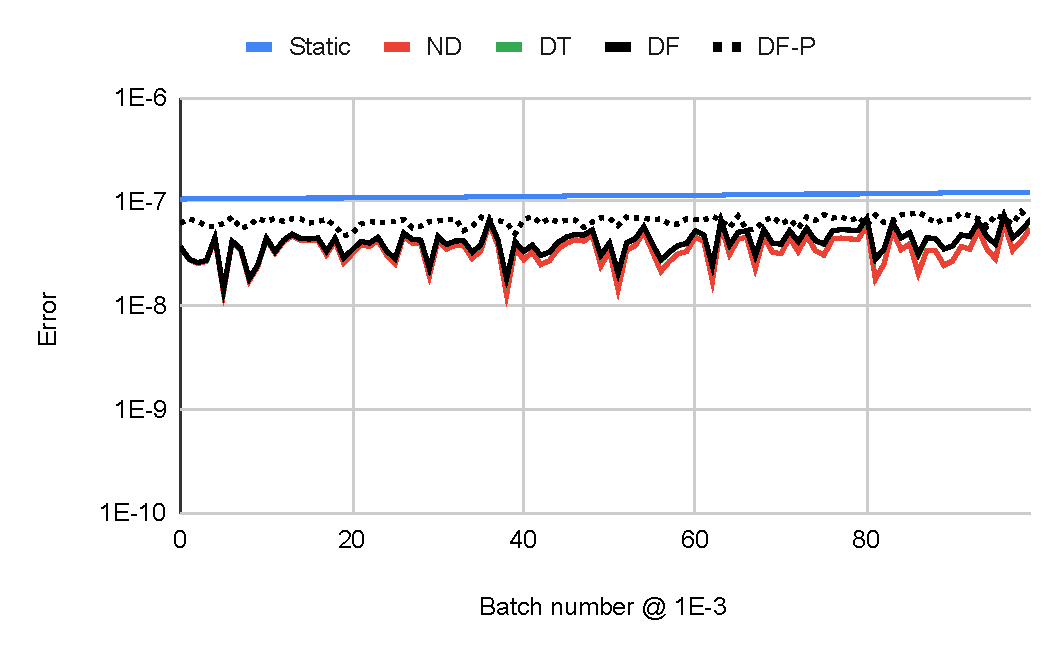
\includegraphics[width=0.48\linewidth]{out/temporal-sx-askubuntu-error3.pdf}
  } \\[-2ex]
  \caption{Runtime and Error in ranks obtained with our GPU implementation of \textit{Static}, \textit{Naive-dynamic (ND)}, \textit{Dynamic Traversal (DT)}, \textit{Dynamic Frontier (DF)}, and \textit{Dynamic Frontier with Pruning (DF-P)} PageRank on the \textit{sx-askubuntu} dynamic graph. The size of batch updates range from $10^{-5}|E_T|$ to $10^{-3}|E_T|$. The rank error with each approach is measured relative to ranks obtained with a reference Static PageRank run, as detailed in Section \ref{sec:measurement}.}
  \label{fig:temporal-sx-askubuntu}
\end{figure*}

\begin{figure*}[!hbt]
  \centering
  \subfigure[Runtime on consecutive batch updates of size $10^{-5}|E_T|$]{
    \label{fig:temporal-sx-superuser--runtime5}
    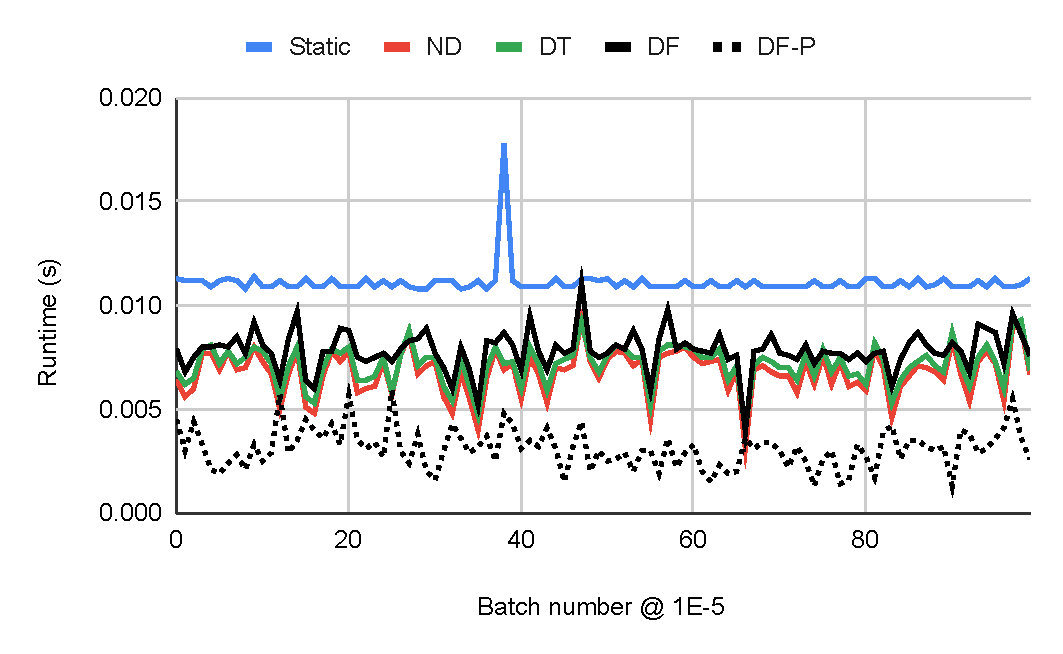
\includegraphics[width=0.48\linewidth]{out/temporal-sx-superuser-runtime5.pdf}
  }
  \subfigure[Error in ranks obtained on consecutive batch updates of size $10^{-5}|E_T|$]{
    \label{fig:temporal-sx-superuser--error5}
    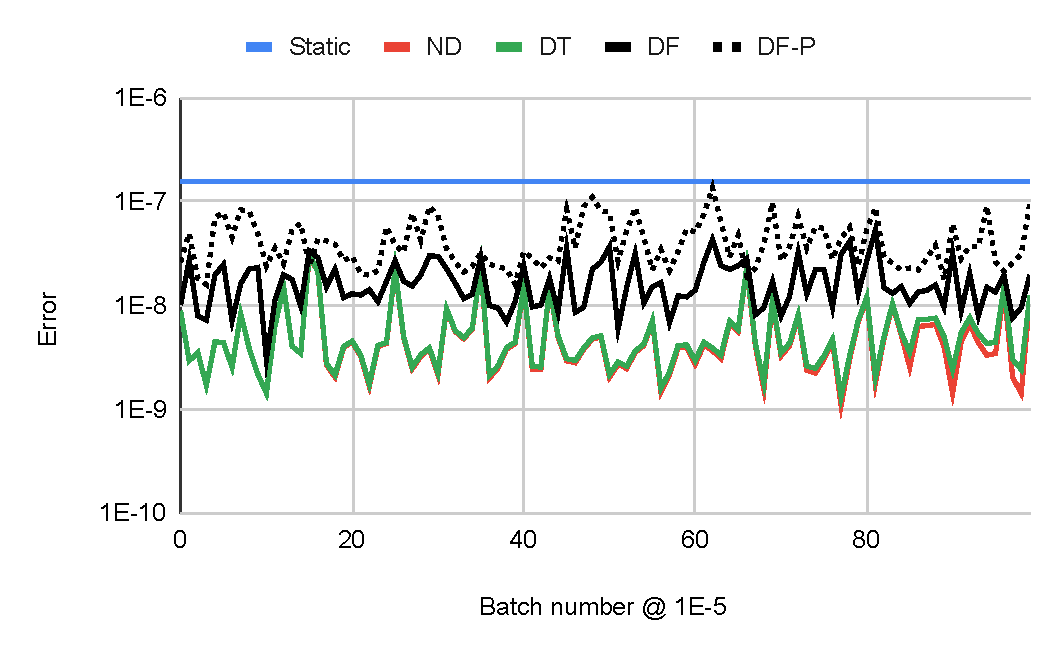
\includegraphics[width=0.48\linewidth]{out/temporal-sx-superuser-error5.pdf}
  } \\[2ex]
  \subfigure[Runtime on consecutive batch updates of size $10^{-4}|E_T|$]{
    \label{fig:temporal-sx-superuser--runtime4}
    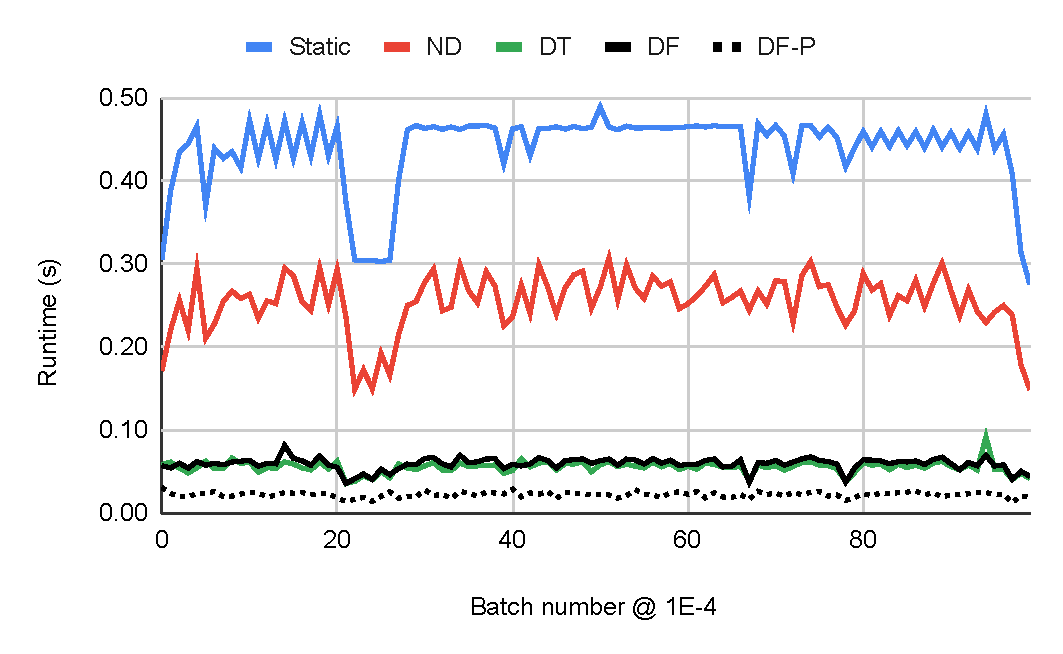
\includegraphics[width=0.48\linewidth]{out/temporal-sx-superuser-runtime4.pdf}
  }
  \subfigure[Error in ranks obtained on consecutive batch updates of size $10^{-4}|E_T|$]{
    \label{fig:temporal-sx-superuser--error4}
    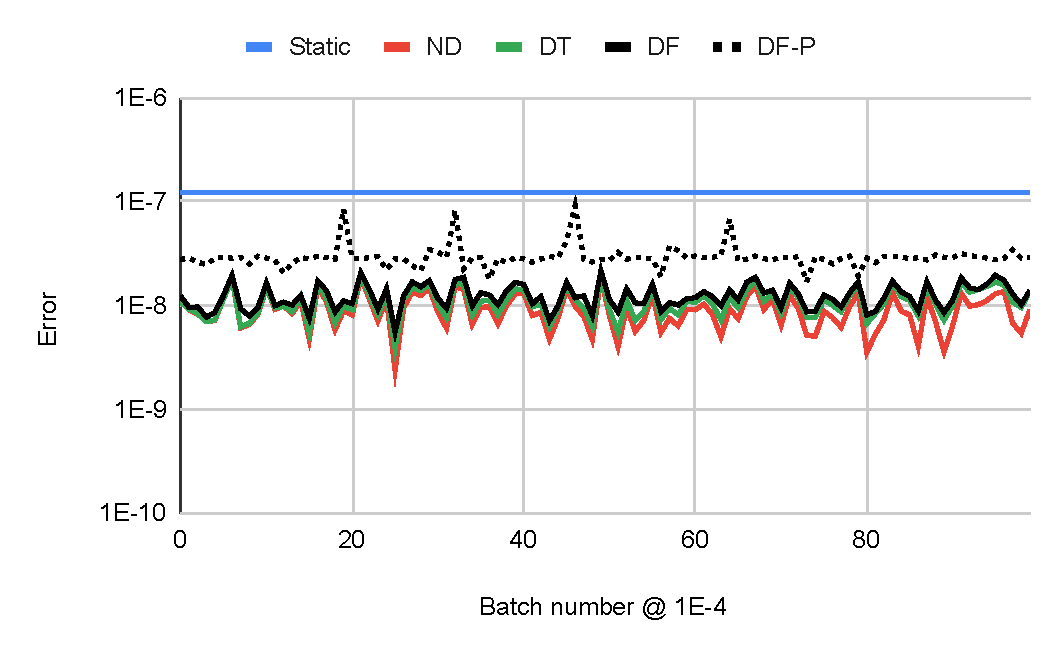
\includegraphics[width=0.48\linewidth]{out/temporal-sx-superuser-error4.pdf}
  } \\[2ex]
  \subfigure[Runtime on consecutive batch updates of size $10^{-3}|E_T|$]{
    \label{fig:temporal-sx-superuser--runtime3}
    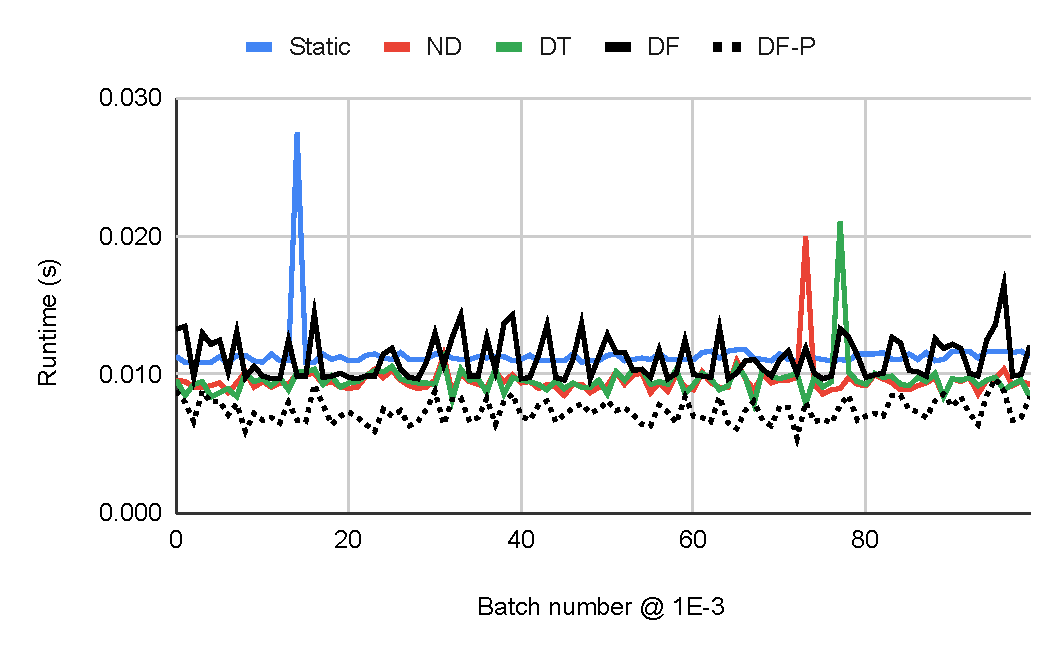
\includegraphics[width=0.48\linewidth]{out/temporal-sx-superuser-runtime3.pdf}
  }
  \subfigure[Error in ranks obtained on consecutive batch updates of size $10^{-3}|E_T|$]{
    \label{fig:temporal-sx-superuser--error3}
    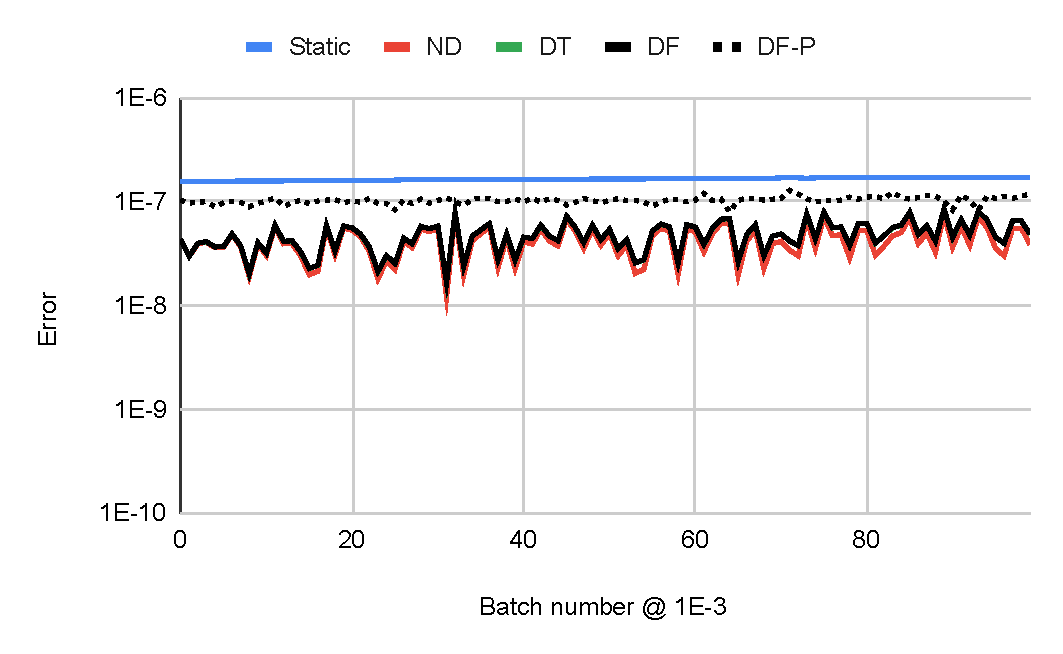
\includegraphics[width=0.48\linewidth]{out/temporal-sx-superuser-error3.pdf}
  } \\[-2ex]
  \caption{Runtime and Error in ranks obtained with \textit{Static}, \textit{Naive-dynamic (ND)}, \textit{Dynamic Traversal (DT)}, our improved \textit{Dynamic Frontier (DF)}, and our improved \textit{Dynamic Frontier with Pruning (DF-P)} PageRank on the \textit{sx-superuser} dynamic graph. The size of batch updates range from $10^{-5}|E_T|$ to $10^{-3}|E_T|$. The rank error with each approach is measured relative to ranks obtained with a reference Static PageRank run, as detailed in Section \ref{sec:measurement}.}
  \label{fig:temporal-sx-superuser}
\end{figure*}

\begin{figure*}[!hbt]
  \centering
  \subfigure[Runtime on consecutive batch updates of size $10^{-5}|E_T|$]{
    \label{fig:temporal-wiki-talk-temporal--runtime5}
    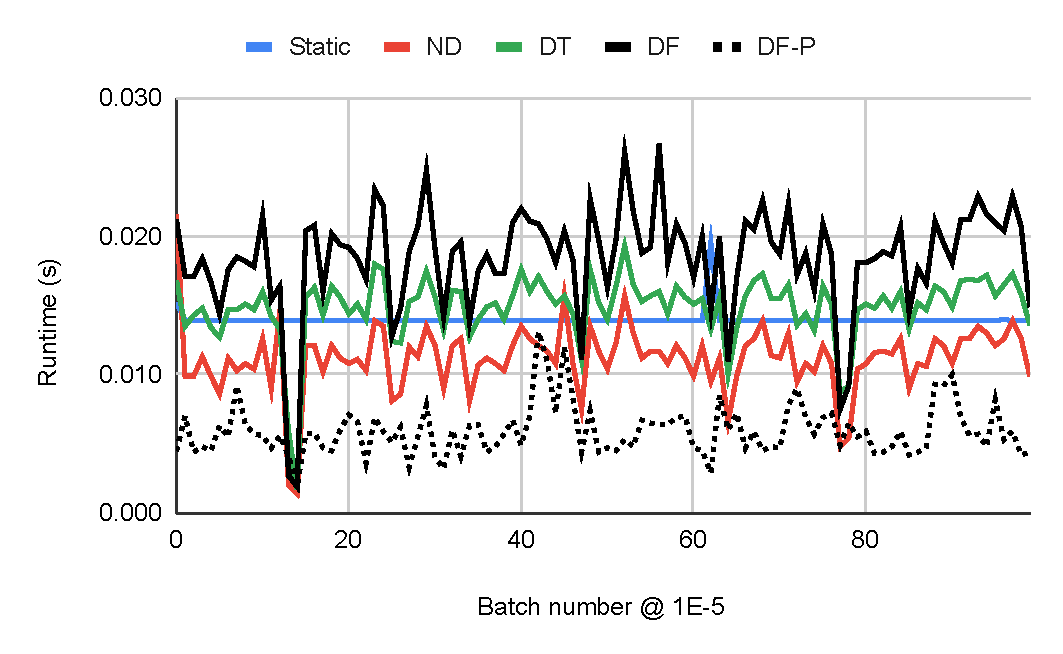
\includegraphics[width=0.48\linewidth]{out/temporal-wiki-talk-temporal-runtime5.pdf}
  }
  \subfigure[Error in ranks obtained on consecutive batch updates of size $10^{-5}|E_T|$]{
    \label{fig:temporal-wiki-talk-temporal--error5}
    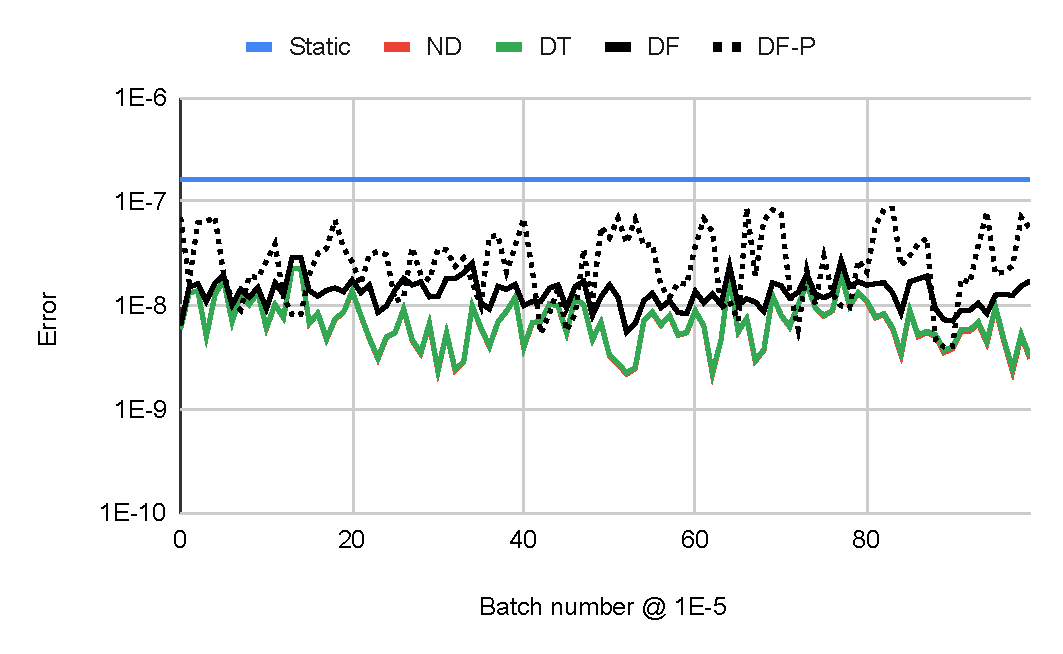
\includegraphics[width=0.48\linewidth]{out/temporal-wiki-talk-temporal-error5.pdf}
  } \\[2ex]
  \subfigure[Runtime on consecutive batch updates of size $10^{-4}|E_T|$]{
    \label{fig:temporal-wiki-talk-temporal--runtime4}
    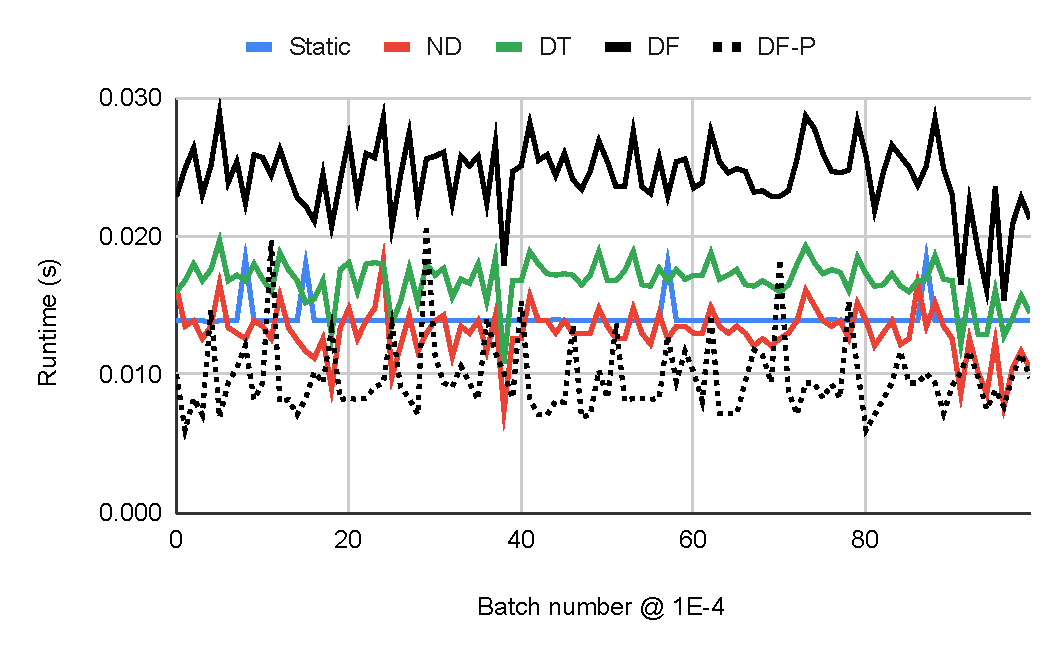
\includegraphics[width=0.48\linewidth]{out/temporal-wiki-talk-temporal-runtime4.pdf}
  }
  \subfigure[Error in ranks obtained on consecutive batch updates of size $10^{-4}|E_T|$]{
    \label{fig:temporal-wiki-talk-temporal--error4}
    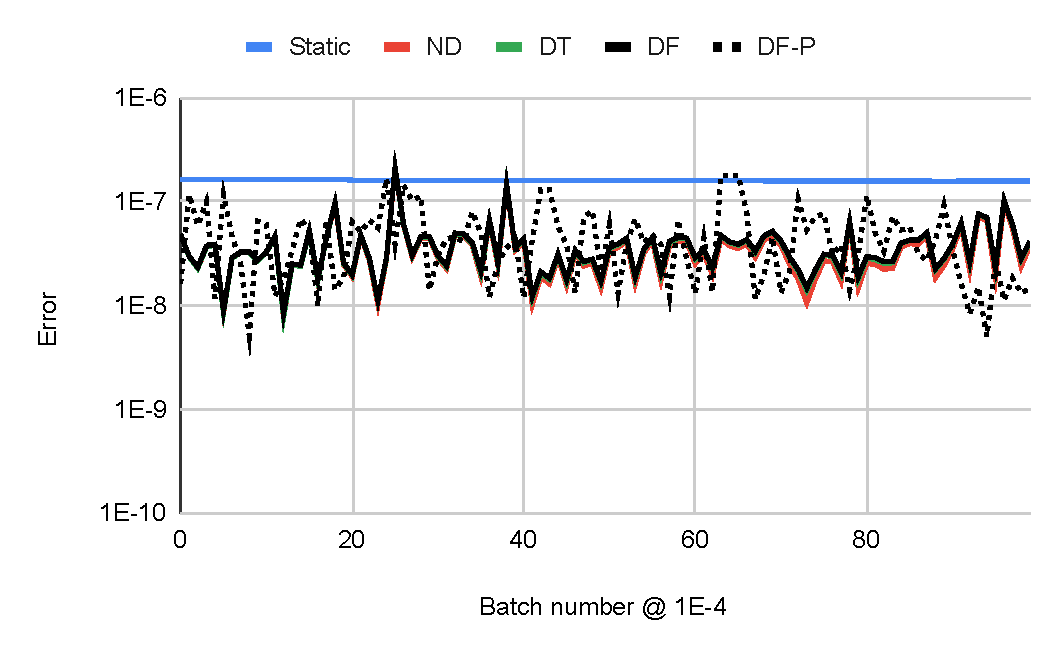
\includegraphics[width=0.48\linewidth]{out/temporal-wiki-talk-temporal-error4.pdf}
  } \\[2ex]
  \subfigure[Runtime on consecutive batch updates of size $10^{-3}|E_T|$]{
    \label{fig:temporal-wiki-talk-temporal--runtime3}
    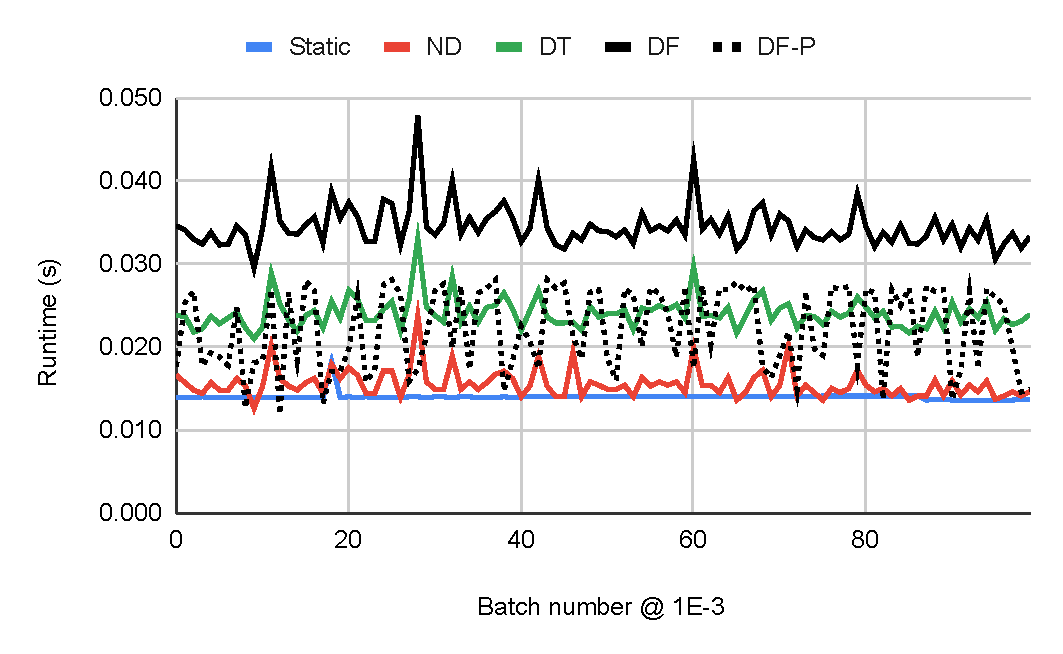
\includegraphics[width=0.48\linewidth]{out/temporal-wiki-talk-temporal-runtime3.pdf}
  }
  \subfigure[Error in ranks obtained on consecutive batch updates of size $10^{-3}|E_T|$]{
    \label{fig:temporal-wiki-talk-temporal--error3}
    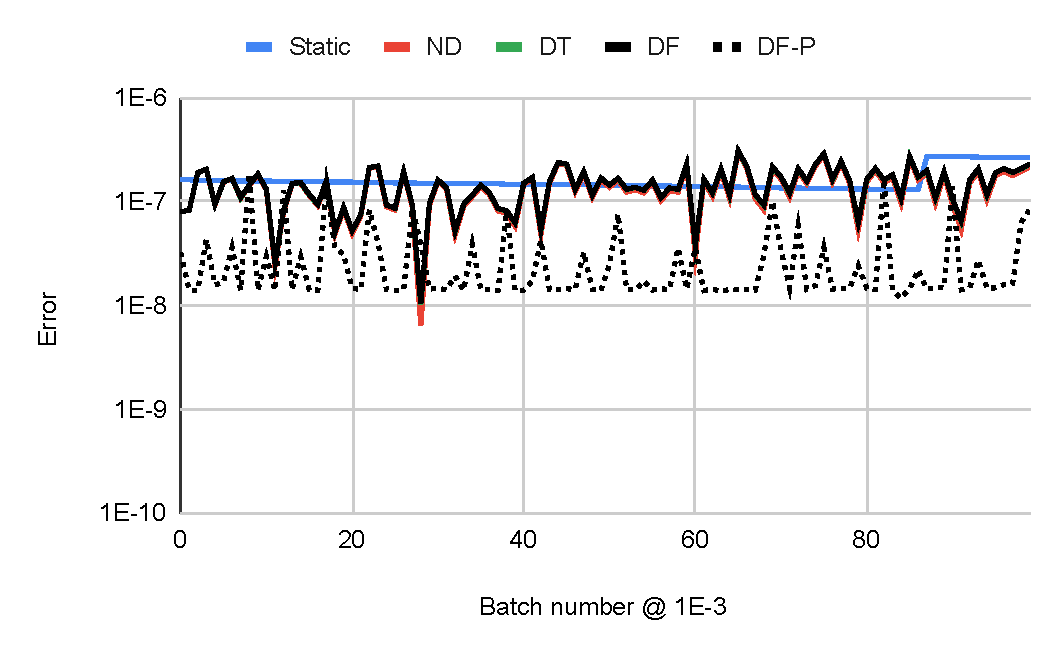
\includegraphics[width=0.48\linewidth]{out/temporal-wiki-talk-temporal-error3.pdf}
  } \\[-2ex]
  \caption{Runtime and Error in ranks obtained with our GPU implementation of \textit{Static}, \textit{Naive-dynamic (ND)}, \textit{Dynamic Traversal (DT)}, \textit{Dynamic Frontier (DF)}, and \textit{Dynamic Frontier with Pruning (DF-P)} PageRank on the \textit{wiki-talk-temporal} dynamic graph. The size of batch updates range from $10^{-5}|E_T|$ to $10^{-3}|E_T|$. The rank error with each approach is measured relative to ranks obtained with a reference Static PageRank run, as detailed in Section \ref{sec:measurement}.}
  \label{fig:temporal-wiki-talk-temporal}
\end{figure*}

\begin{figure*}[!hbt]
  \centering
  \subfigure[Runtime on consecutive batch updates of size $10^{-5}|E_T|$]{
    \label{fig:temporal-sx-stackoverflow--runtime5}
    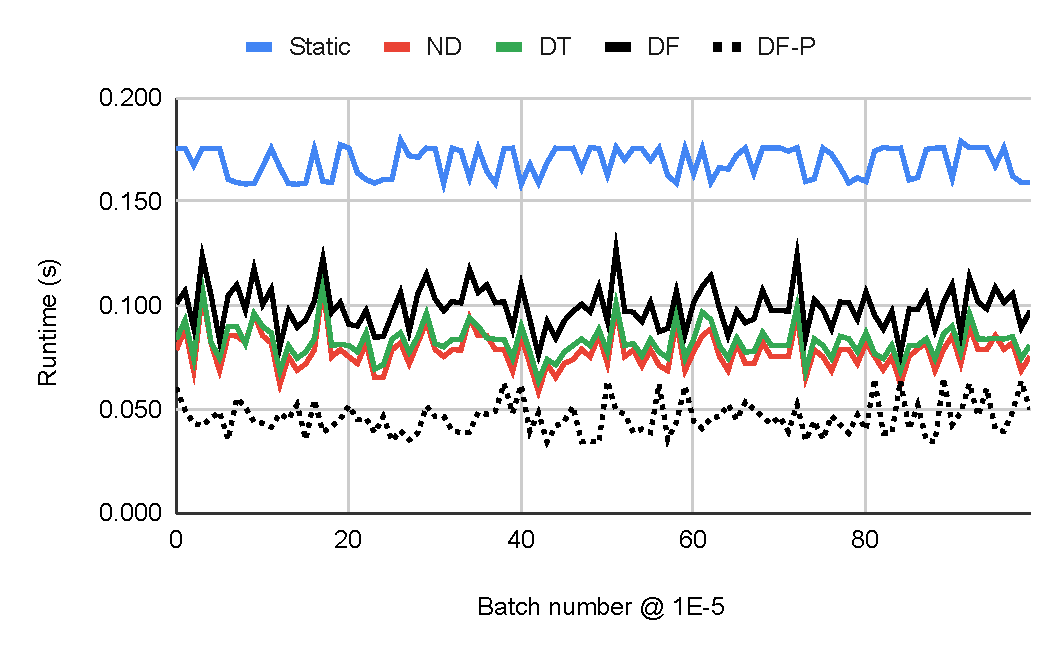
\includegraphics[width=0.48\linewidth]{out/temporal-sx-stackoverflow-runtime5.pdf}
  }
  \subfigure[Error in ranks obtained on consecutive batch updates of size $10^{-5}|E_T|$]{
    \label{fig:temporal-sx-stackoverflow--error5}
    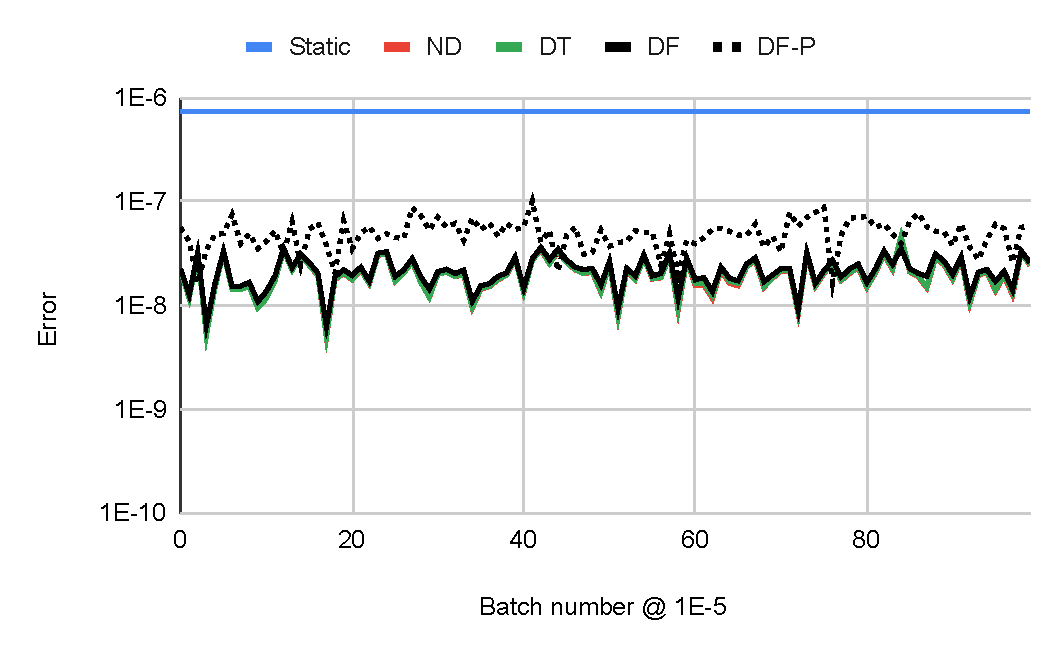
\includegraphics[width=0.48\linewidth]{out/temporal-sx-stackoverflow-error5.pdf}
  } \\[2ex]
  \subfigure[Runtime on consecutive batch updates of size $10^{-4}|E_T|$]{
    \label{fig:temporal-sx-stackoverflow--runtime4}
    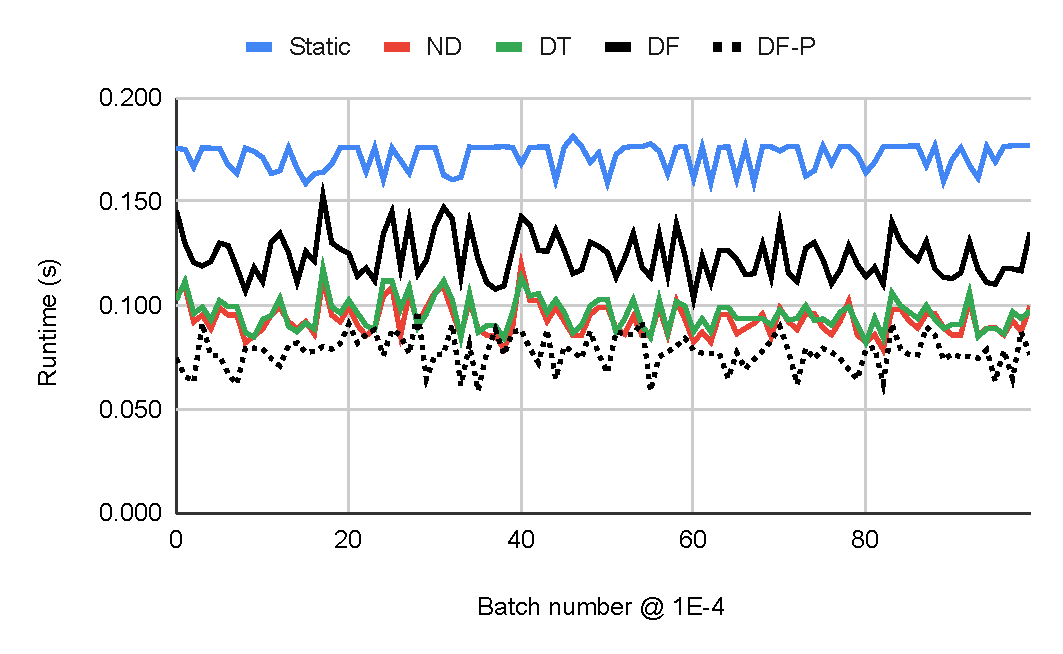
\includegraphics[width=0.48\linewidth]{out/temporal-sx-stackoverflow-runtime4.pdf}
  }
  \subfigure[Error in ranks obtained on consecutive batch updates of size $10^{-4}|E_T|$]{
    \label{fig:temporal-sx-stackoverflow--error4}
    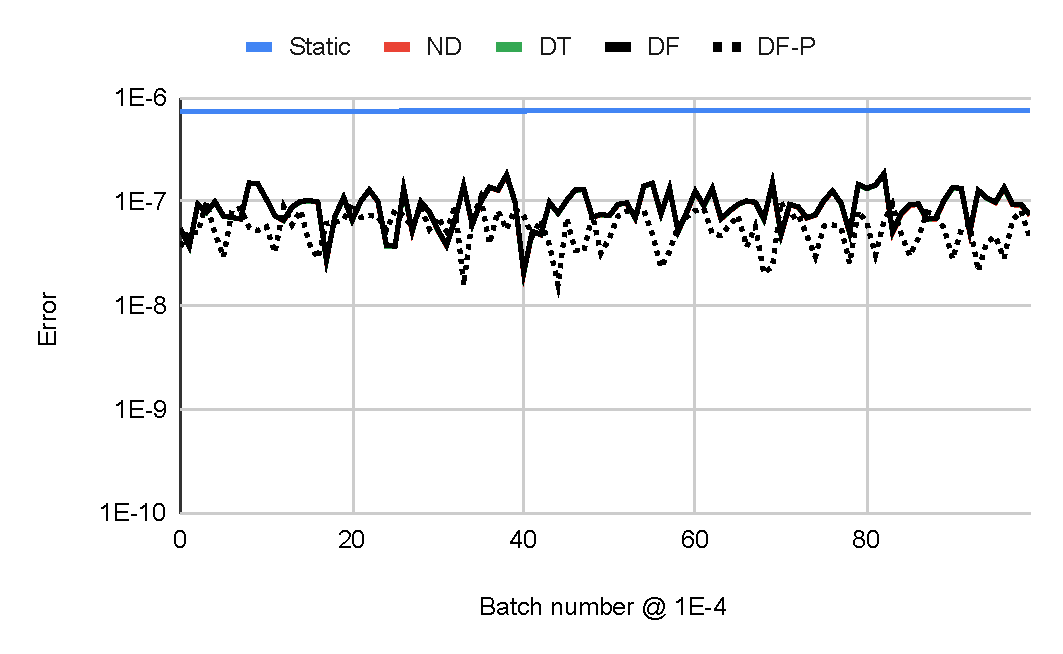
\includegraphics[width=0.48\linewidth]{out/temporal-sx-stackoverflow-error4.pdf}
  } \\[2ex]
  \subfigure[Runtime on consecutive batch updates of size $10^{-3}|E_T|$]{
    \label{fig:temporal-sx-stackoverflow--runtime3}
    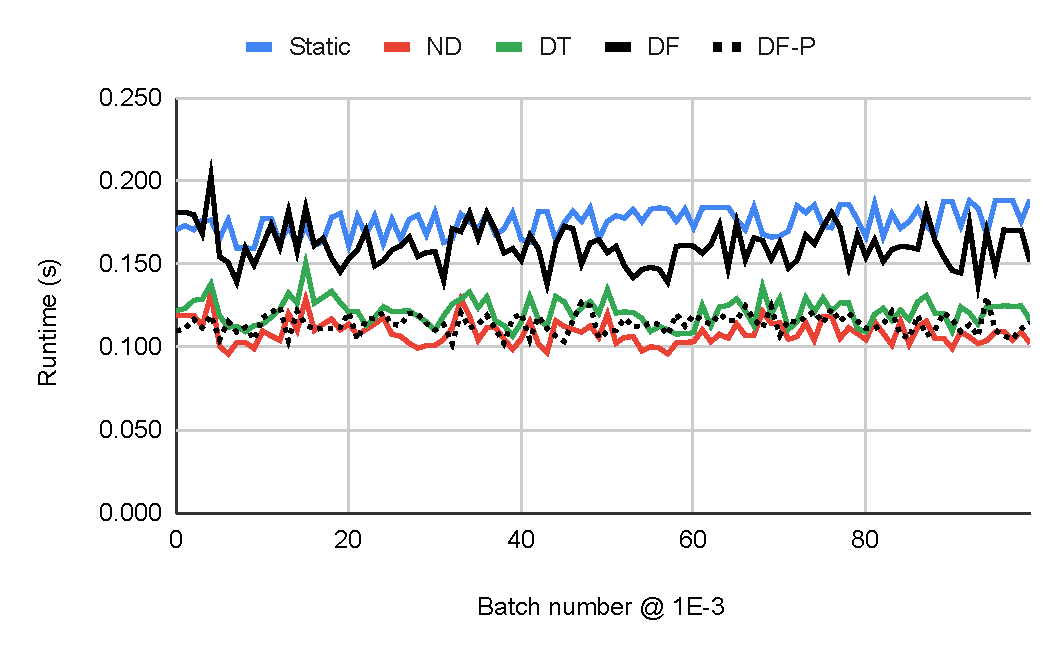
\includegraphics[width=0.48\linewidth]{out/temporal-sx-stackoverflow-runtime3.pdf}
  }
  \subfigure[Error in ranks obtained on consecutive batch updates of size $10^{-3}|E_T|$]{
    \label{fig:temporal-sx-stackoverflow--error3}
    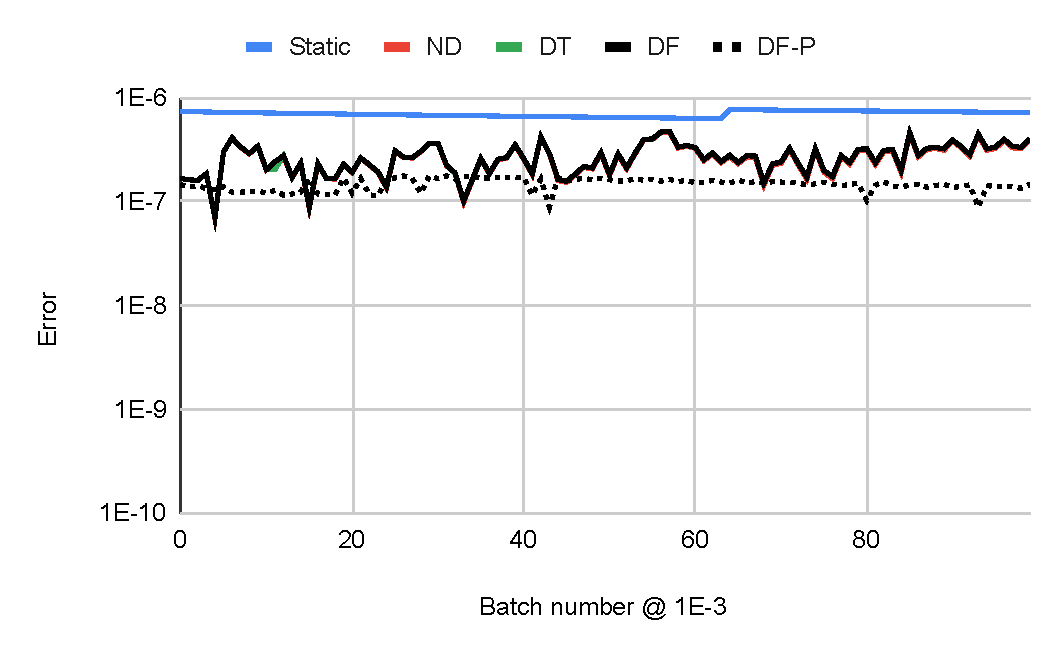
\includegraphics[width=0.48\linewidth]{out/temporal-sx-stackoverflow-error3.pdf}
  } \\[-2ex]
  \caption{Runtime and Error in ranks obtained with \textit{Static}, \textit{Naive-dynamic (ND)}, \textit{Dynamic Traversal (DT)}, our improved \textit{Dynamic Frontier (DF)}, and our improved \textit{Dynamic Frontier with Pruning (DF-P)} PageRank on the \textit{sx-stackoverflow} dynamic graph. The size of batch updates range from $10^{-5}|E_T|$ to $10^{-3}|E_T|$. The rank error with each approach is measured relative to ranks obtained with a reference Static PageRank run, as detailed in Section \ref{sec:measurement}. \su{TOWR}}
  \label{fig:temporal-sx-stackoverflow}
\end{figure*}


\clearpage

\section{Appendix}

\subsection{Derivation of Closed loop formula for Rank calculation towards Dynamic Frontier with Pruning (DF-P) PageRank}
\label{sec:pr-prune-derivation}

We proceed to derive the closed-loop formula for rank calculation with DF-P PageRank. As outlined in Sections \ref{sec:dataset} and \ref{sec:batch-generation}, self-loops are added to each vertex to circumvent the need for a global teleport rank computation in every iteration, thus reducing overhead. In DF-P PageRank, our aim is to skip the computation of ranks for vertices likely to have already converged. However, the existence of self-loops causes a delay in vertex rank convergence due to the immediate recursive nature they introduce. For instance, if the ranks of all in-neighbors of a vertex have already converged, the presence of self-loops inhibits the convergence of the vertex's rank in a single iteration. Nevertheless, we can mitigate this convergence issue by employing a closed-loop formula for the rank calculation of each vertex.

To achieve this, let us denote $r_0$ as the initial rank of a vertex $v$, $\alpha$ as the damping factor, $c = \sum_{u \in G.in(v)\ |\ u \neq v} \frac{R[u]}{|G.out(u)|}$ as the total rank contribution from its in-neighbors (excluding itself), $d = |G.out(v)|$ as its out-degree, and $C_0$ as $1 - \alpha/|V|$. Given the assumption that the rank contribution of its in-neighbors remains constant, the rank of $v$ after one iteration can be expressed as:

\begin{flalign*}
  r_1 & = \alpha (c + \frac{r_0}{d}) + C_0 && \\
      & = \alpha c + \alpha \frac{r_0}{d} + C_0 && \\
\end{flalign*}

\noindent
After the second iteration, the rank of the vertex would be:

\begin{flalign*}
  r_2 & = \alpha (c + \frac{r_1}{d}) + C_0 && \\
      & = \alpha (c + \frac{1}{d} (\alpha c + \alpha \frac{r_0}{d} + C_0)) + C_0 && \\
      & = \alpha c + \alpha^2 \frac{c}{d} + \alpha^2 \frac{r_0}{d^2} + \alpha \frac{C_0}{d} + C_0 &&
\end{flalign*}

\noindent
Following the third iteration, the vertex's rank would be:

\begin{flalign*}
  r_3 & = \alpha (c + \frac{r_2}{d}) + C_0 && \\
      & = \alpha (c + \frac{1}{d} (\alpha c + \alpha^2 \frac{c}{d} + \alpha^2 \frac{r_0}{d^2} + \alpha \frac{C_0}{d} + C_0) + C_0 && \\
      & = \alpha c + \alpha^2 \frac{c}{d} + \alpha^3 \frac{c}{d^2} + \alpha^3 \frac{r_0}{d^3} + \alpha^2 \frac{C_0}{d^2} + \alpha \frac{C_0}{d} + C_0 && \\
\end{flalign*}

\noindent
Expanding this to an infinite number of iterations, the vertex's final rank would be:

\begin{flalign*}
  r_\infty & = \frac{\alpha c}{1 - \alpha / d} + \frac{C_0}{1 - \alpha / d} && \\
           & = \frac{1}{1 - \alpha / d} (\alpha c + C_0)
\end{flalign*}

\noindent
Hence, the closed-loop formula for calculating the rank of a vertex $v$ in DF-P PageRank is:

\begin{flalign}
  R[v] & = \frac{1}{1 - \alpha / |G.out(v)|} \left(\alpha K + \frac{1 - \alpha}{|V|}\right) && \\
    \text{where, } K & = \left(\sum_{u \in G.in(v)} \frac{R[u]}{|G.out(u)|}\right) - \frac{R[v]}{|G.out(v)|}
\end{flalign}

\begin{table}[hbtp]
  \centering
  \caption{List of $12$ graphs sourced from the SuiteSparse Matrix Collection \cite{suite19}, where directed graphs are indicated with $*$. Here, $|V|$ denotes the number of vertices, $|E|$ represents the number of edges (inclusive of self-loops), and $D_{avg}$ represents the average degree.}
  \label{tab:dataset-large}
  \begin{tabular}{|c||c|c|c|c|}
    \toprule
    \textbf{Graph} &
    \textbf{\textbf{$|V|$}} &
    \textbf{\textbf{$|E|$}} &
    \textbf{\textbf{$D_{avg}$}} \\
    \midrule
    \multicolumn{4}{|c|}{\textbf{Web Graphs (LAW)}} \\ \hline
    indochina-2004$^*$ & 7.41M & 199M & 26.8 \\ \hline  % & \num{4.7e-4}
    % uk-2002$^*$ & 18.5M & 311M & 16.8 \\ \hline  % & \num{9.6e-5}
    arabic-2005$^*$ & 22.7M & 654M & 28.8 \\ \hline  % & \num{5.5e-4}
    uk-2005$^*$ & 39.5M & 961M & 24.3 \\ \hline  % & \num{9.6e-5}
    webbase-2001$^*$ & 118M & 1.11B & 9.4 \\ \hline  % & \num{7.3e-7}
    it-2004$^*$ & 41.3M & 1.18B & 28.5 \\ \hline  % & \num{3.8e-4}
    sk-2005$^*$ & 50.6M & 1.98B & 39.1 \\ \hline  % & \num{5.8e-4}
    \multicolumn{4}{|c|}{\textbf{Social Networks (SNAP)}} \\ \hline
    com-LiveJournal & 4.00M & 73.4M & 18.3 \\ \hline  % & \num{7.9e-4}
    com-Orkut & 3.07M & 237M & 77.3 \\ \hline  % & \num{6.7e-2}
    \multicolumn{4}{|c|}{\textbf{Road Networks (DIMACS10)}} \\ \hline
    asia\_osm & 12.0M & 37.4M & 3.1 \\ \hline  % & \num{8.4e-4}
    europe\_osm & 50.9M & 159M & 3.1 \\ \hline  % & \num{6.6e-4}
    \multicolumn{4}{|c|}{\textbf{Protein k-mer Graphs (GenBank)}} \\ \hline
    kmer\_A2a & 171M & 531M & 3.1 \\ \hline  % & \num{9.4e-5}
    kmer\_V1r & 214M & 679M & 3.2 \\ \hline  % & \num{3.2e-4}
  \bottomrule
  \end{tabular}
\end{table}

